\chapter{Financial Projections}

In Joseph Hadzima's MIT OpenCourseWare course, Steve Durzynski takes over just after the financing panel and asks the next unavoidable question: once we know the customer, the business model, the team, and the legal form, what resources does the venture actually need in order to live? This companion chapter, curated by LazyingArt LLC, follows that sequence closely. We move from the motivational turn -- why projections matter at all -- into venture arithmetic, the standard financial statements, the bottom-up construction of a model, the end-state four-year profit-and-loss view, the quarterly cash-flow recurrence, and only then the late pivot to equity, dilution, vesting, and control. The lecture's discipline is simple to state and difficult to evade: the model is not a ceremonial prediction, but a device for forcing assumptions, costs, timing, and risk into the open.

\section{Why We Need Financial Projections}

The lecture opens with a handoff, and the handoff matters. We have already discussed customers, business model, team formation, and legal structure. Only now do we ask what resources the venture will actually require. Durzynski also takes a moment to establish his stance. He is not presenting himself as a pure accountant; he is an engineer and repeat founder explaining why even an engineer must learn to love the model. This is important because the lecture begins from resistance, not from compliance.

That resistance is familiar. The founder says: I am too busy for this; the numbers will be wrong anyway; the investors know every chart goes up and to the right; why not let an accountant do it later? Durzynski does not wave this away. He reverses it. Precisely because the venture is uncertain, the founder needs the model. The model is not introduced as paperwork. It is introduced as a survival instrument.

His governing metaphor is exact and memorable: cash is the oxygen of the venture. We may survive without many things for a while, but not without oxygen. Once that point is accepted, the model ceases to be decorative. It becomes the scorecard for the firm's condition, the roadmap for future spending, and the vehicle by which outside capital is obtained. Investors, lenders, and financially trained listeners want more than upside. They want evidence that we understand the business well enough to describe assumptions, drivers, milestones, and risks.

A compact way to express the operating pressure is through burn:
\begin{equation}
\mathrm{BurnRate} = \mathrm{MonthlyOperatingLoss} + \mathrm{CapitalExpenditures}.
\end{equation}
This is not yet a complete accounting system, but it is already managerial arithmetic. Once we know what we lose each month and what capital equipment we must buy, we are much closer to the central practical question: how long can we keep breathing?

The lecture insists on something else as well. This understanding cannot be outsourced in any meaningful early-stage sense. One may later hire accountants and eventually bring in a CFO, but the founder has to develop a direct feel for the business. What is the average selling price? What is the gross margin? How expensive is the research team? What happens to spending once selling begins? Which milestone failure becomes a cash failure? Durzynski's point is that a good spreadsheet is valuable not because it predicts the future with precision, but because it forces us to ask the right questions with precision.

\subsection{Question \& Answer}

\paragraph{Question.}
Why do financial projections matter if they are going to be wrong anyway?

\paragraph{Answer.}
Because the point is not to be right in every detail. The point is to know what would have to be true for the business to survive and grow. A model that is later revised can still be useful if it has already forced us to identify cost drivers, hiring needs, cash burn, milestones, and downside risk. A founder who refuses to model is not avoiding error; he is avoiding contact with the structure of the business.

\section{Investor Arithmetic Before Accounting}

Only after cash has been established as the binding constraint does the lecture pivot into the numbers investors care about. This is the right order. Before we learn the full bookkeeping machinery, we first need to understand what kind of business can support venture capital at all.

A venture fund has obligations to its own limited partners. That is why not every good small business is venture fundable. A company that grows too slowly may be an excellent business for its founders and still fail the venture test. The point is arithmetic rather than moral judgment. Durzynski gives the lecture's clean rule of thumb:
\begin{equation}
(1+r)^5 = 4
\qquad \Rightarrow \qquad
r \approx 0.32.
\end{equation}
A four-times return in five years corresponds to an internal rate of return of roughly \(32\%\). The lecture uses this as a heuristic, not as a theorem, but the operational meaning is clear: if the slope of the future curve is too shallow, the company may simply be in the wrong financing category.

The time horizon is also part of the arithmetic. A series A investor typically wants a return in something like three to five years, while earlier investors often wait longer. The lecture is careful here: sectors such as medical devices may legitimately require longer plans because regulation and time-to-market are longer. But the underlying logic is unchanged. We are always being asked what eventual path makes the investment worthwhile.

The ownership formula is then stated in its simplest form. If an investor puts in \(I\) dollars at a pre-money valuation \(V_{\mathrm{pre}}\), the post-money valuation is
\begin{equation}
V_{\mathrm{post}} = V_{\mathrm{pre}} + I,
\end{equation}
and the fraction sold in that round is
\begin{equation}
f = \frac{I}{V_{\mathrm{pre}} + I}.
\end{equation}

\paragraph{Worked example.}
If we raise \(\$1\text{M}\) at a \(\$4\text{M}\) pre-money valuation, then
\begin{equation}
f = \frac{1}{4+1} = \frac{1}{5} = 20\%.
\end{equation}
The investor owns one-fifth of the company after the round, and the post-money valuation is \(\$5\text{M}\).

Durzynski then turns immediately to dilution, because ownership in one round is only the beginning of the story. In his example,
\begin{align}
f_A &= \frac{5}{5+5} = 50\%, \\
f_B &= \frac{10}{15+10} = 40\%.
\end{align}
The second round dilutes the holders from the first round. If the first investor held \(50\%\), then after the later \(40\%\) round that stake becomes
\begin{align}
\omega_{A,\mathrm{after}\ B} &= 0.50(1-0.40)=0.30, \\
\omega_{\mathrm{VC,total}} &= 0.30 + 0.40 = 0.70.
\end{align}
So after the two rounds the venture investors together own about \(70\%\) of the business.

Now the lecture makes its most important arithmetic move. The problem is no longer only dilution; it is scale. If investors have put in \(\$15\text{M}\) and want something like \(4\times\) to \(6\times\) back, then their stake must eventually be worth about \(\$60\text{M}\) to \(\$90\text{M}\). Using the lecture's \(70\%\) ownership figure, the implied exit value is on the order of
\begin{equation}
V_{\mathrm{exit}} \approx \frac{60\text{M}}{0.70}\ \text{to}\ \frac{90\text{M}}{0.70}
\approx 86\text{M to }129\text{M}.
\end{equation}
The transcript is unstable around the exact spoken number, so one should read this as cautious reconstruction rather than exact quotation. The key point is that after such financing the company must plausibly reach tens of millions of revenue and a correspondingly large exit value. The more money raised, the higher the bar.

This is why Durzynski is suspicious of the celebratory tone around fundraising. A round is not merely a badge of honor. It is a claim on the future. He says this several ways: the bar keeps moving up; more capital means more has to be achieved; and the right amount of funding is therefore a hard balancing act rather than a simple maximization problem.

\subsection{Question \& Answer}

\paragraph{Question.}
If raising money sounds like success, why does it also make success harder?

\paragraph{Answer.}
Because the round buys runway and reduces immediate risk, but it also installs a larger future obligation. New investors own a fraction of the company and expect that fraction to be worth a large multiple later. So the absolute size of the eventual outcome must rise with the capital raised. A press release may celebrate \(\$5\text{M}\) or \(\$15\text{M}\) raised; the lecture asks us instead what revenue scale and exit value now have to exist for that financing to have made sense.

\section{Reading the Business Through Standard Financials}

Only now do we get the standard set of financial statements. The order is pedagogically deliberate. Durzynski wants us to see formal accounting as the language in which the business model becomes visible, not as a separate discipline dropped on top of it afterward.

\paragraph{Income statement.}
The income statement, or profit-and-loss statement, is the part everyone thinks they know: show revenue, subtract cost of goods sold, and compute what remains. In the lecture's simplified operating language,
\begin{align}
\mathrm{GrossMargin}_t &= R_t - \mathrm{COGS}_t, \\
\mathrm{OperatingProfit}_t &= R_t - \mathrm{COGS}_t - \mathrm{DeptExp}_t.
\end{align}
Here \(R_t\) is revenue, \(\mathrm{COGS}_t\) is cost of goods sold, and \(\mathrm{DeptExp}_t\) is the rollup of departmental expenses: sales, marketing, R\&D, G\&A, staffing, and the rest of the operating structure.

\paragraph{Balance sheet.}
The balance sheet carries assets, liabilities, and equity. Cash is an asset, but so are patents, equipment, and other property. Debts sit on the liability side. Equity is the residual ownership claim. This becomes essential later, when the class turns to the cap table and Durzynski explains that equity ownership belongs to this side of the firm's description, not to the revenue line.

\paragraph{Cash-flow statement.}
The cash-flow statement is where money actually enters and leaves. Durzynski treats it more visually than doctrinally: money comes in, money goes out, and the level rises and falls. That is already enough to see why profit is not identical to survival.

The lecture then shifts from absolute dollars to normalized percentages. Boards and investors often compare firms through ratios because the scale of firms changes rapidly but the percentage signature of a business model is often recognizable. We therefore define
\begin{equation}
\mathrm{GrossMarginPct}_t = \frac{\mathrm{GrossMargin}_t}{R_t},
\qquad
\mathrm{OpMargin}_t = \frac{\mathrm{OperatingProfit}_t}{R_t}.
\end{equation}
Different businesses leave different ratio fingerprints.

This is why Durzynski shows old-school hardware and software examples. A hardware company with very low R\&D and low operating profit tells one story; a software firm with higher R\&D, higher SG\&A, and higher eventual margins tells another. Joe Hadzima's intervention sharpens the point: if our numbers differ greatly from successful comparable businesses, then either we do not understand the business model or we must explain why ours is economically different.

The lecture's rules of thumb are therefore not identities but comparison standards, especially for the year-four view:
\begin{equation}
\frac{\mathrm{R\&D}}{R} \approx 10\%\text{--}20\%,
\qquad
\frac{\mathrm{G\&A}}{R} \approx 5\%\text{--}15\%,
\qquad
\frac{\mathrm{OperatingProfit}}{R} \approx 15\%\text{--}20\%.
\end{equation}
Durzynski is careful to say that these are not meant for the earliest chaotic quarters. Year one in a startup is often too distorted by ramp-up and loss. But by the year-four view the ratio structure should begin to resemble something a pattern-matching investor can recognize.

There is also a practical asymmetry in the lecture's treatment of margins. Operating expenses can sometimes be squeezed. Gross margin is harder to repair because it is usually baked into the product or service itself. That is why the lecture treats gross margin as a particularly revealing number.

\section{Building the Model From the Bottom Up}

Having taught us how to read the business, the lecture now turns to how we construct it. The pace becomes more practical. We are no longer looking at statements from above; we are asking what cells, hires, prices, and contracts have to be entered to make those statements emerge.

The model begins with very concrete questions. What exactly is the product or service? What price will it command? What is the unit cost of manufacturing or delivery? What overhead is required to support it? How is it sold: direct, through partners, through distributors, or through an internal sales force that does not yet exist?

One of the lecture's clearest small examples contrasts direct sale and distributor sale. If the nominal sale price is \(100\), then in the direct case the company books the full sale price as revenue:
\begin{equation}
\mathrm{BookedRevenue}_{\mathrm{direct}} = 100.
\end{equation}
In the distributor case, the distributor takes \(20\) off the top, so the company books
\begin{equation}
\mathrm{BookedRevenue}_{\mathrm{distributor}} = 100 - 20 = 80.
\end{equation}
The tradeoff is immediate. Revenue booked is lower, but so is the burden of direct selling. The spreadsheet is useful precisely because such strategic choices show up immediately in the numbers.

The lecture is equally plain that in the earliest phase the founders themselves are often the first salespeople. That is more than folklore. It means the model cannot jump from zero to scale by magic. We have to ask how the first customer is obtained, then the second, then the tenth. We have to ask what the sales cycle is, how much support must be promised, whether support contracts renew, and how long it takes a new salesperson to become productive.

Durzynski then opens the KPI layer. Churn, committed monthly recurring revenue, customer acquisition cost, lifetime value, and the ratio \(\mathrm{LTV}/\mathrm{CAC}\) are not presented as decorative dashboard numbers. They are mechanisms by which a business may decide whether injecting more capital into customer acquisition actually creates value. In one audience exchange, this becomes a useful two-box distinction. There is an operating box and an investment box. An operating dollar might be modeled very roughly as
\begin{equation}
1 \mapsto 1.10,
\end{equation}
while a venture investor thinks in far larger equity multiples. The boxes are different, but linked: a better operating machine can make the equity stake much more valuable.

Staffing then enters as the dominant driver of departmental expense. Durzynski uses simple operating heuristics:
\begin{equation}
\mathrm{Benefits} \approx 0.15 \times \mathrm{Salary},
\qquad
\mathrm{DeptExp}_{\mathrm{staff}} \approx 0.67 \times \mathrm{TotalExpenses}.
\end{equation}
Most early burn is people. That is why the lecture spends real time on salary determination, minimum viable founder salary, and market-based compensation for key hires. A founder should not starve, but should not use newly raised capital as personal extraction. The lecture's language is memorable: investors do not want you to starve, but they do want you to be hungry.

There is also an instructive exchange about whether a single product-level NPV or positive-value argument is enough. The lecture answers no. A positive product unit economics story is only a kernel. Around it must sit infrastructure, rent, hiring, marketing, manufacturing, and the rest of the corporation. In the very earliest sketch, average-cost approximations may be fine. But once real capital is being raised to be spent on real people, the model must become granular.

Durzynski is equally sharp about tools. Business-planning software is not recommended as a substitute for understanding, and AI is treated cautiously. It may help us brainstorm KPIs or strategic variants, but it cannot relieve us of the obligation to understand how the spreadsheet works. If we cannot explain why the cells are what they are, then the model is not really ours.

Finally, the lecture returns to the central forecasting discipline: build sales from the bottom up. Start with one sale, then two, then the cadence of a real sales process. Do not begin by declaring that there are billions of people in the world and we will take \(1\%\) of them. Yet bottom-up does not mean blind. There must still be a market-size reality check. If the bottom-up forecast implies owning more than the market, the model has failed in a different direction.

\subsection{Question \& Answer}

\paragraph{Question.}
Why is a bottom-up sales forecast more credible than a large market-share story?

\paragraph{Answer.}
Because a bottom-up forecast exposes mechanism. It forces us to say who buys, at what price, through which channel, on what timetable, with what staffing, and at what cost. A large-market story usually hides all of that beneath a percentage of an enormous total. Investors do not fund market size; they fund sales machinery. A defendable forecast is one whose gears can be named.

\section{From Assumptions to the Four-Year P\&L}

The lecture now makes one of its strongest structural moves: start with the end in mind. Instead of opening every worksheet tab first, Durzynski shows the finished four-year profit-and-loss output. This is not a shortcut. It is a way of fixing our attention on the visible outcome investors care about before we descend into the machinery that produces it.

\begin{figure}[t]
\centering

\includegraphics[width=0.96\linewidth]{lecture_08_figure_02.png}
\caption{Four-year P\&L forecast with revenue and operating profit.}
\end{figure}

The slide is a summary chart rather than a derivation board, and that is precisely why it is so useful. Revenue rises steeply across the four years. Operating profit begins below zero, approaches the axis by Year 2, and is clearly positive by the later years. The lecture uses this picture to condense several thoughts into one visual object: top-line growth, delayed profitability, and the finite amount of cash that must be survived before break-even.

\begin{figure}[t]
\centering
\begin{tikzpicture}[x=1.6cm,y=0.12cm]
\draw[->] (0,-28) -- (0,80);
\draw[->] (0,0) -- (4.3,0);

\draw (0,-25) -- (4.0,-25);
\draw (0,25) -- (4.0,25);
\draw (0,50) -- (4.0,50);
\draw (0,75) -- (4.0,75);

\node[anchor=east] at (-0.08,-25) {\$-25};
\node[anchor=east] at (-0.08,0) {\$0};
\node[anchor=east] at (-0.08,25) {\$25};
\node[anchor=east] at (-0.08,50) {\$50};
\node[anchor=east] at (-0.08,75) {\$75};

\node at (0.8,-31) {Year 1};
\node at (1.8,-31) {Year 2};
\node at (2.8,-31) {Year 3};
\node at (3.8,-31) {Year 4};

\draw[thick,red] (0.8,2) -- (1.8,12) -- (2.8,38) -- (3.8,66);
\draw[thick,blue] (0.8,-4) -- (1.8,-2) -- (2.8,7) -- (3.8,16);

\node[anchor=west] at (3.85,66) {Revenue};
\node[anchor=west] at (3.85,16) {Operating Profit};
\end{tikzpicture}
\caption{Qualitative redraw of the four-year forecast. The geometry is schematic rather than numerically exact.}
\end{figure}

This picture allows Durzynski to make a very useful inference. If we sum the negative operating results before break-even, we estimate how much cash the company needs in order to survive until profitability. The lecture gives a concrete arithmetic version:
\begin{equation}
\mathrm{CashNeed}_{\mathrm{pre\mbox{-}BE}} \approx 3.3\text{M} + 2.6\text{M}
\approx 5.9\text{M} \approx 6\text{M}.
\end{equation}
The chart suggests the same thing geometrically:
\begin{equation}
\mathrm{CashNeed}_{\mathrm{pre\mbox{-}BE}}
\approx
\int_{\mathrm{OperatingProfit}(t)<0}
-\mathrm{OperatingProfit}(t)\,dt.
\end{equation}
The lecture uses this only as intuition -- an ``integral under the curve'' way of seeing cumulative early losses -- not as a claim that the slide itself gives precise continuous data. But the conceptual move is exactly right. The losses before break-even are the cash burden that must be financed.

This is why Durzynski does not stop at the minimum. If the curve suggests \(\$6\text{M}\) of pre-break-even need, he still recommends raising more, perhaps \(\$10\text{M}\), so there is room for delays and mistakes. The model is not only an argument for future profitability. It is an estimate of how much uncertainty the venture can survive.

The lecturer also reads the slope of the red revenue curve for a rough sense of growth quality. The transcript is unstable around the term he uses there, and one should not formalize it too aggressively. The safe point is simpler: the chart is not read only for whether profit becomes positive. It is read for how quickly the business seems to scale once it begins to move.

\subsection{Question \& Answer}

\paragraph{Question.}
If the company loses money in the first years, what exactly makes the model credible?

\paragraph{Answer.}
Not the smoothness of the graph by itself. Credibility comes from the path underneath the graph: units sold, selling price, channel choice, support retention, manufacturing cost, hiring plan, rent, overhead, and timing. Early losses are acceptable only if the route from those losses to later profitability can be explained in operational detail. The graph compresses the story; it does not replace the story.

\section{Cash Flow, CAPEX, and the Timing of Survival}

After the annual and quarterly P\&L rollups, the lecture pivots into the cash-flow view. This is where the spreadsheet becomes dynamic. We are no longer asking only whether the business looks profitable eventually. We are asking when cash actually runs low, when the next financing must happen, and how capital expenditure changes the path.

\begin{figure}[t]
\centering

\includegraphics[width=0.96\linewidth]{lecture_08_figure_03.png}
\caption{CAPEX and cash-flow spreadsheet layout.}
\end{figure}

The slide teaches several things at once. First, it gives the row order of the cash model: beginning cash, investment, total revenue, COGS, departmental expenses, capital expense, change in cash, ending balance. Second, it shows that the workbook is modular: lower tables feed upper tables, and the color scheme indicates how the information travels. Third, it gives the reader a practical legend: red means user input, magenta means a link to another sheet, black means calculated value, and blue means a value pulled in from another sheet.

The bookkeeping spine of the slide can be written cleanly as
\begin{align}
\Delta C_q &= I_q + R_q - \mathrm{COGS}_q - \mathrm{DeptExp}_q - \mathrm{CapEx}_q, \\
C_q^{\mathrm{end}} &= C_q^{\mathrm{beg}} + \Delta C_q, \\
C_{q+1}^{\mathrm{beg}} &= C_q^{\mathrm{end}}.
\end{align}
This is the recurrence Durzynski is gesturing toward when he describes the cash level going up and down quarter by quarter. We begin the quarter with cash, add financing and revenue, subtract operating costs and capital spending, and carry what remains into the next quarter.

The lower capital-expense block explains where the capital line comes from. In abstract form,
\begin{equation}
\mathrm{CumCapEx}_q = \sum_{\tau \le q} \mathrm{CapEx}_{\tau}.
\end{equation}
A few entries in the screenshot are legible enough to illustrate the running sum:
\begin{align}
(\mathrm{CapEx}_{Q1},\mathrm{CapEx}_{Q2},\mathrm{CapEx}_{Q3},\mathrm{CapEx}_{Q4},\mathrm{CapEx}_{Q1'})
&=
(84,152,226,288,312)\times 10^3, \\
(\mathrm{CumCapEx}_{Q1},\mathrm{CumCapEx}_{Q2},\mathrm{CumCapEx}_{Q3},\mathrm{CumCapEx}_{Q4},\mathrm{CumCapEx}_{Q1'})
&=
(84,236,462,750,1062)\times 10^3.
\end{align}
These numbers should be read only as clearly visible examples from the slide, not as a full spreadsheet transcription. Their purpose is to show the cumulative logic, not to replace the original evidence.

The cash-flow slide also hints that revenue collection may lag the P\&L by a quarter. The text is not legible enough to formalize that timing in full detail, but the existence of such lag is exactly why cash flow is not reducible to the annual income statement.

\begin{figure}[t]
\centering
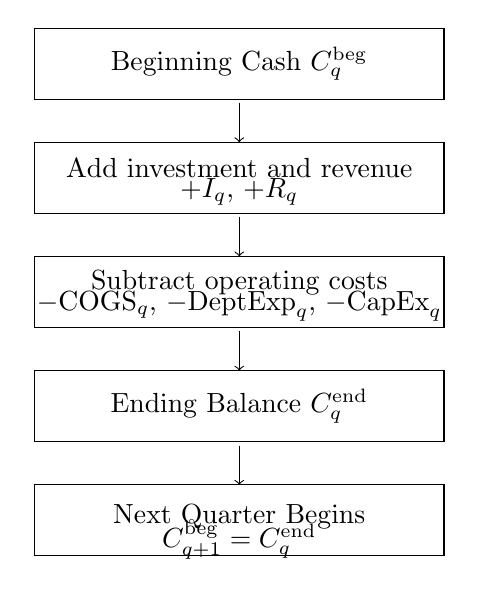
\begin{tikzpicture}[x=1cm,y=1cm]
\draw (0,0) rectangle (5.2,0.9);
\node at (2.6,0.45) {Beginning Cash $C_q^{\mathrm{beg}}$};

\draw[->] (2.6,-0.05) -- (2.6,-0.55);

\draw (0,-1.45) rectangle (5.2,-0.55);
\node at (2.6,-0.88) {Add investment and revenue};
\node at (2.6,-1.18) {$+I_q$, $+R_q$};

\draw[->] (2.6,-1.5) -- (2.6,-2.0);

\draw (0,-2.9) rectangle (5.2,-2.0);
\node at (2.6,-2.33) {Subtract operating costs};
\node at (2.6,-2.63) {$-\mathrm{COGS}_q$, $-\mathrm{DeptExp}_q$, $-\mathrm{CapEx}_q$};

\draw[->] (2.6,-2.95) -- (2.6,-3.45);

\draw (0,-4.35) rectangle (5.2,-3.45);
\node at (2.6,-3.90) {Ending Balance $C_q^{\mathrm{end}}$};

\draw[->] (2.6,-4.40) -- (2.6,-4.90);

\draw (0,-5.80) rectangle (5.2,-4.90);
\node at (2.6,-5.30) {Next Quarter Begins};
\node at (2.6,-5.60) {$C_{q+1}^{\mathrm{beg}} = C_q^{\mathrm{end}}$};
\end{tikzpicture}
\caption{Cash-flow recurrence implied by the workbook structure.}
\end{figure}

Durzynski's spoken walkthrough makes the recurrence concrete. Start with zero. Add \(\$5\text{M}\) of investment. Spend through the quarter. End with roughly \(\$4\text{M}\). Carry that amount into the next quarter. Spend again. If the balance falls toward a dangerous floor, then the next raise has to happen before the floor is reached. In the lecture's example, that means raising more money before the company drops below a comfortable cash threshold.

This is why cash flow is operationally more useful than many founders first assume. Some conversations, especially high-level investor conversations, will focus on the income statement. But survival is a timing problem, and the cash-flow table is where timing becomes explicit. The model is no longer merely asking whether the business can become profitable someday. It is asking whether the company can stay alive long enough to reach that someday.

\section{Presentation Discipline and the Late Pivot to Equity}

Once the model exists, the lecture turns to presentation. The first principle is that the model is iterative. It should be beaten up by friends, advisors, and investors. The point of that beating-up is not humiliation. The point is to discover which assumptions break first, and what has to be changed if they do.

At the executive-summary level, the lecture recommends an annual P\&L with percentages so that investors can pattern-match the business quickly. In deeper due diligence, one may need the full structure: annual P\&L, quarterly P\&L, staffing plan, quarterly cash flow, and the assumptions behind pricing, hiring, profitability timing, and cash need. Large firms may bring in finance professionals of their own to push on the weak points of the model.

The lecture is equally disciplined about what not to show too early. One should know the biggest risks and have backup material ready. One should model what happens if milestones slip or key hires are delayed. But one should not lead the pitch deck with best-case and worst-case scenarios. The founder is being asked to show conviction in a base case, and then to defend that case under questioning. Risk scenarios belong more naturally in the appendix or in live discussion.

Only after this financial spine is in place does Durzynski pivot to equity. This ordering matters. The pie is not split in a vacuum. It is split after we understand what sort of enterprise is being financed and what kind of work still lies ahead.

The algebra of the cap table is simple:
\begin{equation}
\omega_i = \frac{s_i}{S},
\end{equation}
where \(s_i\) is the share count of holder \(i\) and \(S\) is the total fully diluted share count. The lecture then illustrates, through audience questions, how easy it is to recover valuation from a percentage. If \(\$0.5\text{M}\) buys \(10\%\) of the company, the post-money value is about \(\$5\text{M}\). If \(\$5\text{M}\) buys \(50\%\), the post-money value is about \(\$10\text{M}\). If \(\$10\text{M}\) is raised on a \(\$15\text{M}\) pre-money valuation, then the post-money value is \(\$25\text{M}\). These are just late-stage reappearances of the same financing arithmetic from earlier in the lecture.

The lecture then adds vesting, because raw ownership without time commitment is unstable. A standard four-year schedule with a one-year cliff can be written as
\begin{equation}
v(m)=
\begin{cases}
0, & 0 \le m < 12, \\
0.25 + \dfrac{0.75}{36}(m-12), & 12 \le m \le 48, \\
1, & m \ge 48.
\end{cases}
\end{equation}
Nothing vests during the first year. At month 12, one-quarter vests. The remaining three-quarters vest monthly across the next 36 months. Durzynski's rationale is direct: much of the most valuable work is still in the future, so ownership has to remain attached to future contribution.

The cap-table examples are then read as a sequence of dilutions. Founders begin with a simple split. Key employees and advisors are added. An angel round arrives. An option pool is created, diluting existing holders even before the later investor shares are issued. Then larger venture rounds arrive and dilution accelerates. The lecture is concrete here: after enough rounds, a founding CEO may be down in the neighborhood of \(10\%\) to \(15\%\), and if dilution becomes too severe the incentive structure can break. Boards sometimes respond by re-upping a founder's compensation package precisely because motivation is part of the value of the company.

The lecture also distinguishes advisory roles from board roles. Advisors may receive small grants -- often around a quarter-percent or a half-percent, subject to negotiation and market conditions -- in exchange for support and credibility. But a true board seat carries fiduciary duty and a continuing legal obligation to the corporation. That is why one often works with someone as an advisor before asking them to join the real board.

Durzynski then makes the control distinction explicit. There is equity control and there is board control. These are not the same thing. Preferred stock may carry board access and governance rights that do not appear in a naive percentage table. Hence the lecture's practical closing principle: do not think only about raw percentage. Think about who is at the table, who appoints the independent director, how decisions are made, and whether trust with investors is strong enough to support the company through later rounds. In that spirit he repeats a memorable line: in negotiations of this kind, one wants to be at the table rather than on the menu.

The final practical notes follow naturally. Outside VC financing often brings directors' and officers' insurance. Investor board seats do not normally receive extra equity beyond the investment itself. And because the market for talent changes over time, compensation for senior hires, advisors, and board members remains negotiated rather than fixed by formula. The arithmetic is clean; the actual bargain is not.

\subsection{Question \& Answer}

\paragraph{Question.}
How much of the company can we give away before the founder stops having a meaningful reason to stay?

\paragraph{Answer.}
There is no exact universal threshold in the lecture, and the speaker refuses to pretend otherwise. But the warning is sharp. After enough rounds, a founder can discover that the ownership left on the table no longer feels like a real stake. When that happens, incentive and control begin to separate dangerously. The lecture's response is twofold: first, vesting and option-pool design should reward future contribution; second, boards sometimes have to repair a founder's package if dilution has gone too far. Equity, in this lecture, is never just arithmetic. It is arithmetic tied to motivation, trust, and continued work.

\section{Summary}

The lecture unfolds with more deliberateness than a bare list of topics would suggest. We begin from founder skepticism and answer it with a biological fact: cash is oxygen. We then pass into investor arithmetic, because financing changes the scale of success the business must eventually reach. Next we learn the grammar of the standard financial statements and the ratio language by which investors compare business models. From there we build the model from the bottom up: units, prices, channels, hires, support, overhead, KPIs, and sales timing. Only then do we step back to the four-year P\&L, read its graph as a compressed argument about delayed profitability, and move into the quarterly cash-flow recurrence, where timing becomes the central problem of survival. Finally, and only finally, the lecture turns to equity, vesting, dilution, option pools, board control, and founder incentive. The model is wrong in detail because the future is unknown, but it is indispensable because without it we do not know what we are asking the company to become.